\documentclass[10pt,aspectratio=169]{beamer}

\usetheme{metropolis}

\usepackage{booktabs}
\usepackage{graphicx}
\usepackage{amsmath}
\usepackage{xcolor}
\usepackage{hyperref}
\usepackage{tikz}
\usetikzlibrary{shapes.geometric, arrows.meta, positioning, fit, backgrounds, calc}

\title{Cost-Aware Tracker Blocking in Firefox}
\subtitle{Per-request privacy intervention accounting at browser scale}
\author{James Han}
\institute{Privacy Team \\ Full-Stack Engineering Intern}
\date{April 29, 2026}

\begin{document}

% ============================================================
% 1 - Title
% ============================================================
\begin{frame}
    \titlepage
\end{frame}

% ============================================================
% 2 - What this talk is about
% ============================================================
\begin{frame}{What this talk is about}
    \begin{center}
    \Large
    Firefox serves \textbf{more than 200 million users} worldwide, each blocking thousands of tracker requests per month. \\[1em]
    Our new-tab privacy widget will surface them as \textbf{counts}. \\[1em]
    \textcolor{blue}{This work provides a model that converts those counts into \textbf{costs}.}
    \end{center}

    \vspace{0.6em}
    \small
    \textbf{What we estimate per blocked request:}
    \begin{itemize}
        \item \textbf{Transfer size} -- how many bytes the response would have moved over the wire if Firefox hadn't blocked it
        \item \textbf{Download duration} -- how long pulling those bytes would have taken
    \end{itemize}
    Each is predicted separately. Transfer size is the deployed target; download duration is a secondary metric.
\end{frame}

% ============================================================
% 3 - Today's privacy widget undercounts
% ============================================================
\begin{frame}{Today's privacy widget is undercounting}
    \textbf{Enhanced Tracking Protection (ETP)} is Firefox's tracker blocker. It uses the \textbf{Disconnect list} (an open-source list of tracker domains) to decide what to block. Today the new-tab widget tells the user \textit{how many} were blocked.

    \vspace{0.6em}
    \textbf{But not all blocks are equal:}
    \begin{itemize}
        \item A \texttt{bat.bing.com} tracking pixel: \textbf{258 bytes}, $\sim$5 ms
        \item A \texttt{googletagmanager.com} SDK: \textbf{170 KB}, $\sim$300 ms
        \item Today the widget treats them the same
    \end{itemize}

    \vspace{0.8em}
    \textbf{Three audiences need the cost answer:}
    \begin{itemize}
        \item \textbf{Users} -- what is ETP actually doing for me
        \item \textbf{Blocklist maintainers} -- which rules pull weight
        \item \textbf{Privacy research} -- compare ETP to Brave Shields, Safari ITP, uBlock Origin honestly
    \end{itemize}
\end{frame}

% ============================================================
% 4 - One browsing session (visual)
% ============================================================
\begin{frame}{What a single browsing session looks like today}
    \centering
    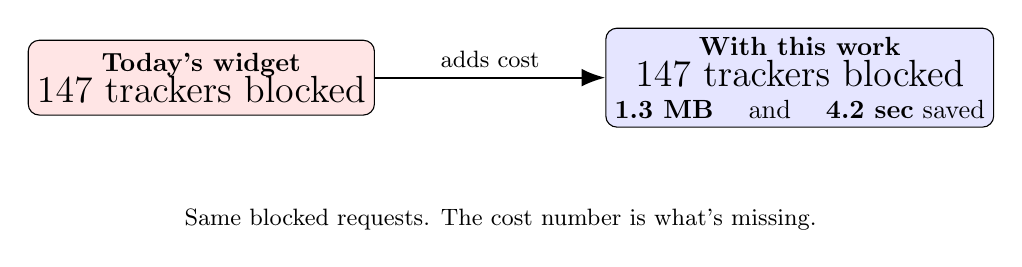
\begin{tikzpicture}[scale=0.95, transform shape]
      % Today
      \node[draw, rounded corners, fill=red!10, minimum width=4.5cm, minimum height=1cm, align=center] (today) at (-4, 1.5) {\textbf{Today's widget}\\\Large 147 trackers blocked};
      % Tomorrow
      \node[draw, rounded corners, fill=blue!10, minimum width=4.5cm, minimum height=1.2cm, align=center] (tomorrow) at (4, 1.5) {\textbf{With this work}\\\Large 147 trackers blocked\\\normalsize \textbf{1.3 MB} \quad and \quad \textbf{4.2 sec} saved};

      % Arrow
      \draw[-{Latex[length=3mm]}, thick] (today.east) -- (tomorrow.west) node[midway, above] {\small adds cost};

      % Caption
      \node at (0, -0.4) {\small Same blocked requests. The cost number is what's missing.};
    \end{tikzpicture}

    \vspace{0.8em}
    \small
    A 30-minute browsing session triggers $\sim$150 tracker blocks. The user sees a count, not a magnitude. Without magnitudes, there's no way to tell whether ETP is doing meaningful work for that user, or whether tightening one rule would matter more than another.
\end{frame}

% ============================================================
% 5 - The catch (we never see the response)
% ============================================================
\begin{frame}{The catch: we blocked the request, so we never see the response}
    \textbf{What the browser sees at block time:}
    \begin{itemize}
        \item URL, resource type (script/image/beacon), initiator (which page asked), HTTP method
    \end{itemize}

    \vspace{0.5em}
    \textbf{What we want to predict (never observed):}
    \begin{itemize}
        \item Transfer size in bytes, download duration in milliseconds
    \end{itemize}

    \vspace{0.7em}
    \textcolor{blue}{The response is \textbf{structurally never received.}}

    \vspace{0.4em}
    \small
    \textit{Counterfactual prediction: estimate the cost of something that didn't happen because we prevented it.}
\end{frame}

% ============================================================
% 6 - Why this is hard (Brave's paired-crawl)
% ============================================================
\begin{frame}{Brave already shipped something. Here's why we did it differently.}
    \textbf{Brave (2019)} ships a bandwidth savings predictor in their browser today. They got there with a shortcut: paired crawls for training labels, page-level prediction.

    \vspace{0.4em}
    \begin{center}
    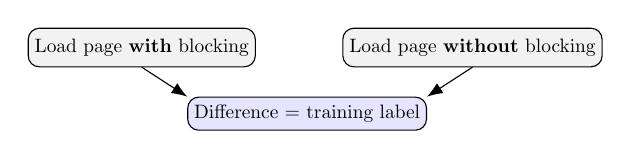
\begin{tikzpicture}[scale=0.7, transform shape]
        \node[draw, rounded corners, minimum width=3.5cm, minimum height=0.7cm, align=center, fill=gray!10] (a) at (-3, 0.7) {Load page \textbf{with} blocking};
        \node[draw, rounded corners, minimum width=3.5cm, minimum height=0.7cm, align=center, fill=gray!10] (b) at (3, 0.7) {Load page \textbf{without} blocking};
        \node[draw, rounded corners, minimum width=4cm, minimum height=0.6cm, align=center, fill=blue!10] (c) at (0, -0.5) {Difference = training label};
        \draw[-{Latex[length=2mm]}] (a.south) -- (c.north west);
        \draw[-{Latex[length=2mm]}] (b.south) -- (c.north east);
    \end{tikzpicture}
    \end{center}

    \vspace{0.3em}
    \textbf{Three problems for our use case:}
    \begin{itemize}
        \item \textbf{Expensive to refresh.} Every training row needs a paired crawl.
        \item \textbf{Less accurate.} $R^2 = 0.68$, median error 2.7 MB per session.
        \item \textbf{Wrong granularity.} Page totals only. Can't say \textit{which tracker} cost the user, or which Disconnect rule pulls weight.
    \end{itemize}

    \vspace{0.4em}
    \tiny
    \textit{Source: ``Accurately Predicting Ad Blocker Savings,'' Brave blog, October 2019.}
\end{frame}

% ============================================================
% 7 - Walking through one tracker request (visual)
% ============================================================
\begin{frame}{One real example: what the model gets and what it predicts}
    \centering
    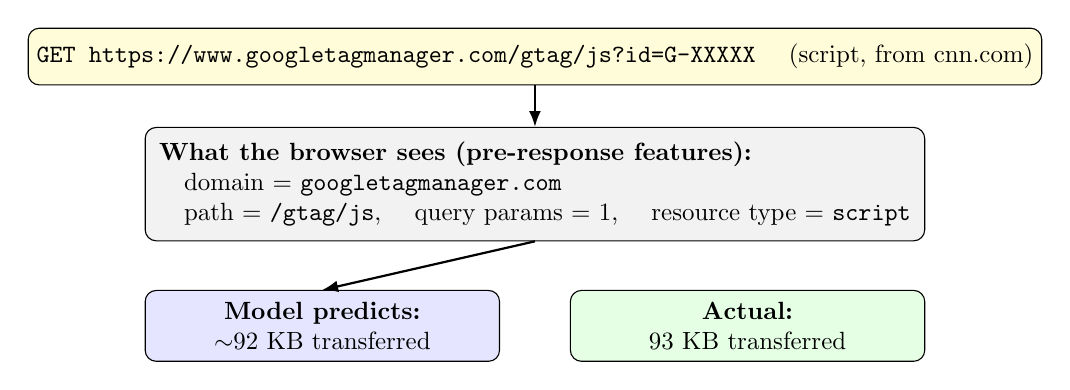
\begin{tikzpicture}[scale=0.9, transform shape]
        % URL box
        \node[draw, rounded corners, fill=yellow!15, minimum width=11cm, minimum height=0.8cm, align=center] (url) at (0, 2.5) {\texttt{GET https://www.googletagmanager.com/gtag/js?id=G-XXXXX} \quad (script, from cnn.com)};

        % Features extracted
        \node[draw, rounded corners, fill=gray!10, minimum width=11cm, minimum height=1.6cm, align=left] (feat) at (0, 0.7) {\textbf{What the browser sees (pre-response features):}\\
        \quad domain = \texttt{googletagmanager.com}\\
        \quad path = \texttt{/gtag/js}, \quad query params = 1, \quad resource type = \texttt{script}};

        % Prediction
        \node[draw, rounded corners, fill=blue!10, minimum width=5cm, minimum height=1cm, align=center] (pred) at (-3, -1.3) {\textbf{Model predicts:}\\$\sim$92 KB transferred};
        \node[draw, rounded corners, fill=green!10, minimum width=5cm, minimum height=1cm, align=center] (act) at (3, -1.3) {\textbf{Actual:}\\93 KB transferred};

        % Arrows
        \draw[-{Latex[length=2mm]}, thick] (url.south) -- (feat.north);
        \draw[-{Latex[length=2mm]}, thick] (feat.south) -- (pred.north);
    \end{tikzpicture}

    \vspace{0.4em}
    \small
    \textit{The browser had this information \textbf{before} blocking. The model converts that information into a cost estimate.}
\end{frame}

% ============================================================
% 8 - Domain-level estimation is wrong
% ============================================================
\begin{frame}{Domain-level estimation is structurally wrong}
    \begin{columns}[T]
    \begin{column}{0.55\textwidth}
        \centering
        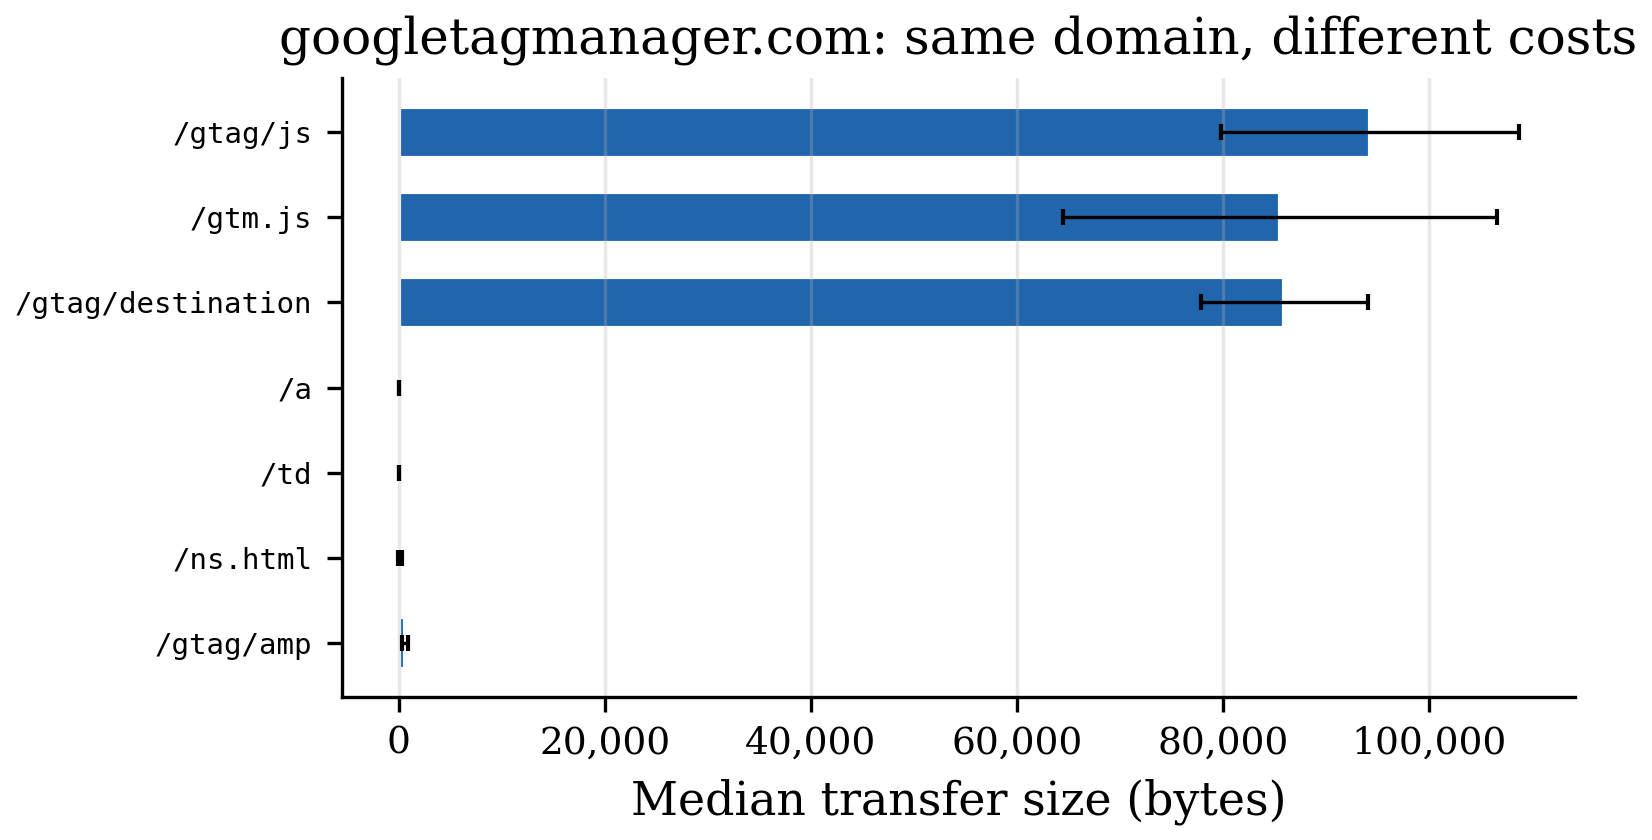
\includegraphics[width=\columnwidth]{figures/fig11_domain_example.pdf}
    \end{column}
    \begin{column}{0.45\textwidth}
        \textbf{Same domain. Three orders of magnitude.}

        \vspace{0.6em}
        \texttt{googletagmanager.com}:
        \begin{itemize}
            \item \texttt{/gtag/js} $\to$ $\sim$93 KB
            \item \texttt{/collect} $\to$ 0 bytes
        \end{itemize}

        \vspace{0.6em}
        Within-domain spread (CV = std-dev/mean): \textbf{0.94 at median}, \textbf{3.0 at p90}.

        \vspace{0.6em}
        Lookup-by-domain cannot tell these apart. \textbf{The URL path is the primary determinant of cost, not the domain.}
    \end{column}
    \end{columns}
\end{frame}

% ============================================================
% 9 - Shape of the data
% ============================================================
\begin{frame}{The shape of the data}
    \centering
    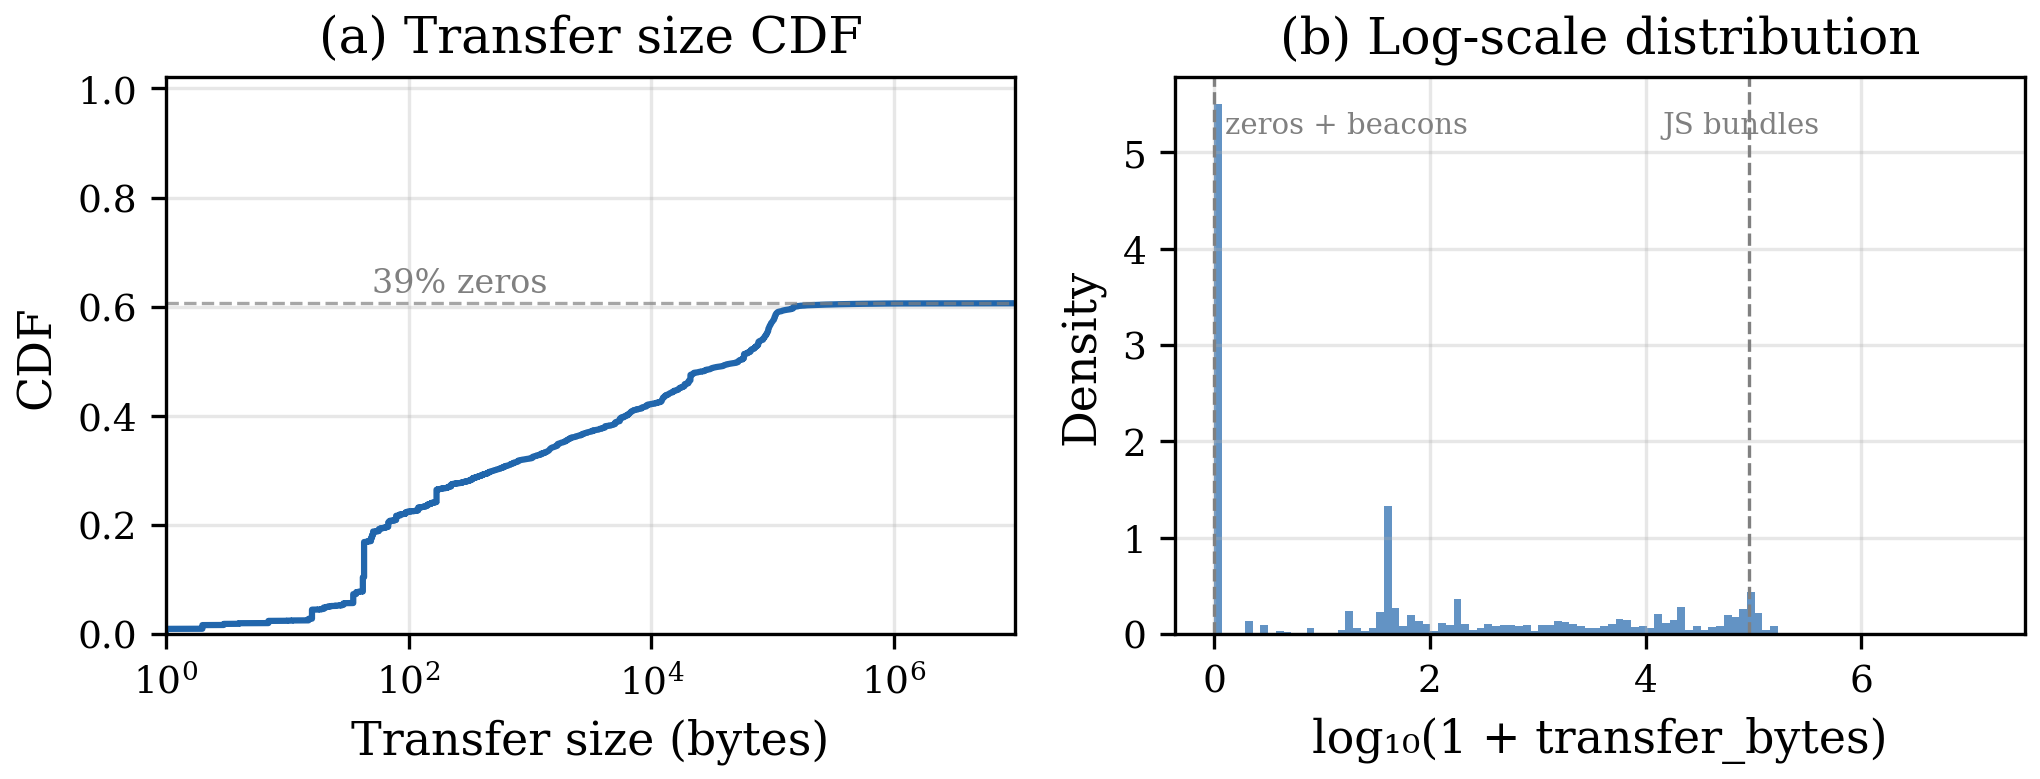
\includegraphics[width=0.78\textwidth]{figures/fig1_target_distribution.pdf}

    \vspace{0.4em}
    \begin{itemize}
        \item \textbf{39.5\% exact zeros} (tracking beacons return nothing — they're "fire and forget")
        \item Heavy right tail out to \textbf{8.6 MB} (giant JavaScript SDKs)
        \item Mean 13.6 KB, median 43 bytes
    \end{itemize}

    \vspace{0.3em}
    \textcolor{blue}{Spike at zero, long tail of large bundles.} \textit{This shape will dictate the loss function later.}
\end{frame}

% ============================================================
% 10 - Data
% ============================================================
\begin{frame}{Data}
    \textbf{HTTP Archive June 2024 mobile crawl} — public dataset of synthetic web crawls run from a fixed test environment. Filtered to third-party tracker requests in 5 Disconnect categories.

    \vspace{0.8em}
    \begin{center}
        \Large \textbf{3.49M requests}\quad across\quad \textbf{3,723 tracker domains}
    \end{center}

    \vspace{0.8em}
    \textbf{Why training on Chrome data and deploying in Firefox is fine:}

    Transfer size is \textit{server-determined}. The same URL returns the same payload to any browser. Crawl population (Chrome via HTTP Archive) and deployment population (Firefox real users) see different traffic mixes, but the bytes are the bytes.

    \vspace{0.4em}
    \small
    \textit{No domain-adaptation tricks needed.}
\end{frame}

% ============================================================
% 11 - Lookup table vs model (explainer)
% ============================================================
\begin{frame}{Lookup table vs.\ model: a one-slide intuition}
    \centering
    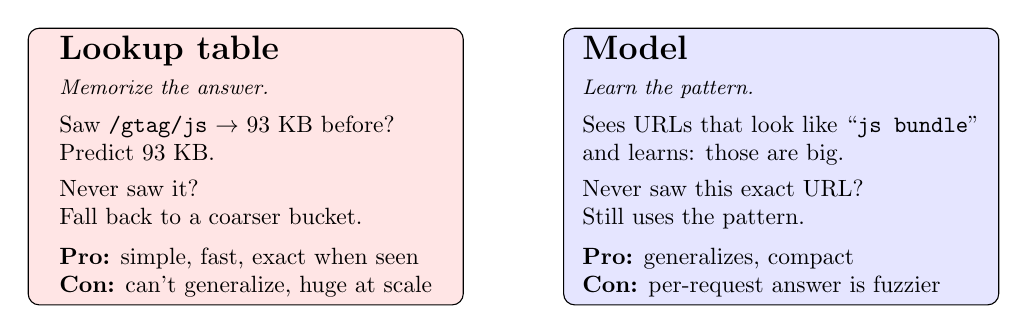
\begin{tikzpicture}[scale=0.85, transform shape]
        % LUT
        \node[draw, rounded corners, fill=red!10, minimum width=6.5cm, minimum height=4cm, align=left] (lut) at (-4, 0) {\textbf{\Large Lookup table}\\[0.3em]
        \small \textit{Memorize the answer.}\\[0.4em]
        Saw \texttt{/gtag/js} $\to$ 93 KB before? \\Predict 93 KB.\\[0.3em]
        Never saw it? \\Fall back to a coarser bucket.\\[0.5em]
        \textbf{Pro:} simple, fast, exact when seen\\
        \textbf{Con:} can't generalize, huge at scale};

        % Model
        \node[draw, rounded corners, fill=blue!10, minimum width=6.5cm, minimum height=4cm, align=left] (mod) at (4, 0) {\textbf{\Large Model}\\[0.3em]
        \small \textit{Learn the pattern.}\\[0.4em]
        Sees URLs that look like ``\texttt{js bundle}'' \\and learns: those are big.\\[0.3em]
        Never saw this exact URL? \\Still uses the pattern.\\[0.5em]
        \textbf{Pro:} generalizes, compact\\
        \textbf{Con:} per-request answer is fuzzier};
    \end{tikzpicture}

    \vspace{0.4em}
    \small
    \textit{We'll see in a moment that the model wins even where the lookup table has the answer memorized.}
\end{frame}

% ============================================================
% 12 - Lookup-table ladder (figure)
% ============================================================
\begin{frame}{First, try the boring thing: lookup tables}
    \begin{columns}[T]
    \begin{column}{0.55\textwidth}
        \centering
        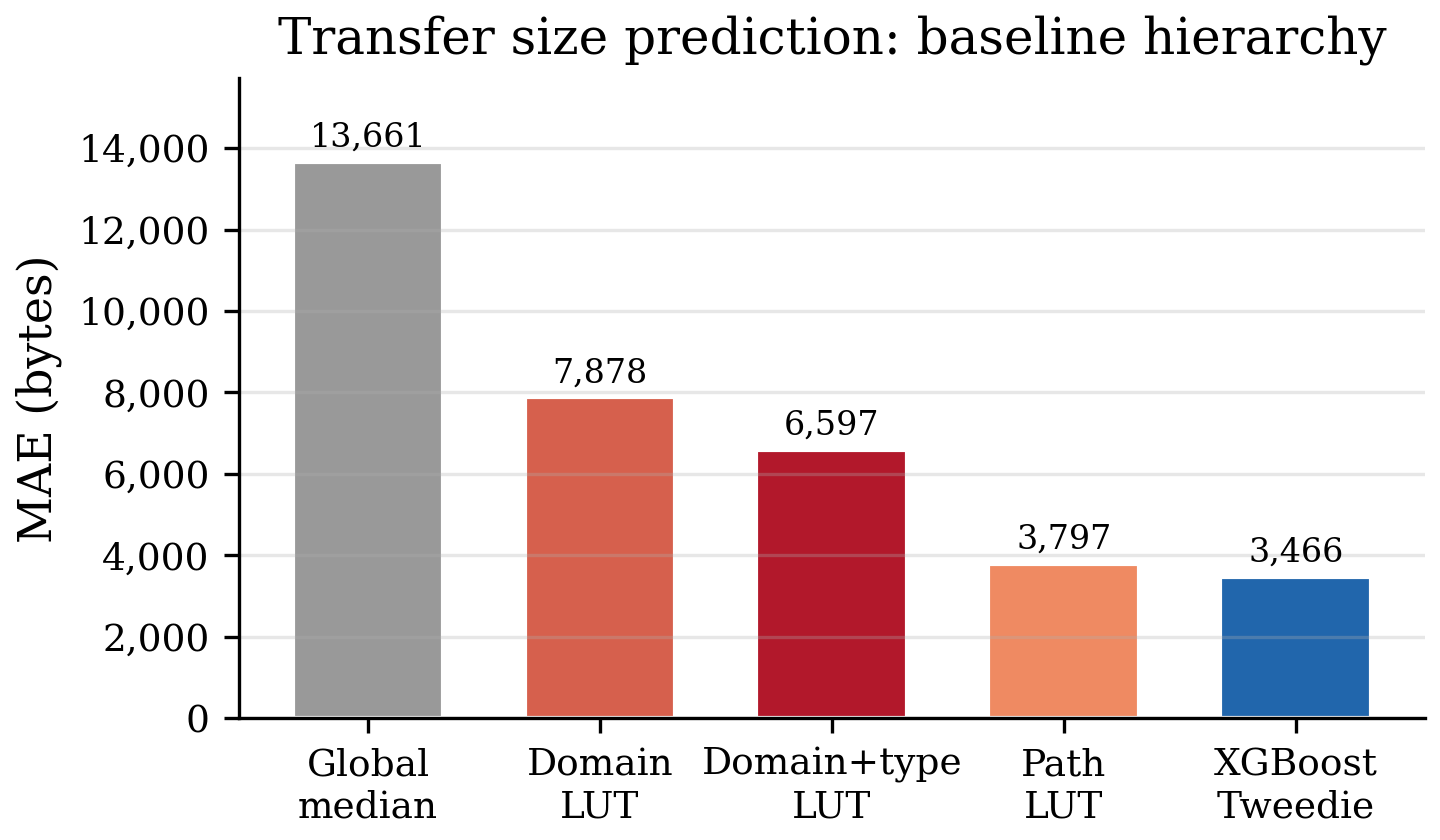
\includegraphics[width=\columnwidth]{figures/fig2_baseline_ladder.pdf}
    \end{column}
    \begin{column}{0.45\textwidth}
        \textbf{Make the lookup key finer, error drops:}
        \begin{itemize}
            \item Global median: 13,661
            \item Domain: 7,878
            \item Domain + type: 6,597
            \item Path: 3,797
            \item \textbf{Our model: 3,466}
        \end{itemize}

        \vspace{0.7em}
        Path LUT looks competitive on offline eval.

        \vspace{0.4em}
        It \textbf{cannot deploy.}
    \end{column}
    \end{columns}
    \small
    \textit{MAE (mean absolute error) = average bytes off per request. Lower is better.}
\end{frame}

% ============================================================
% 13 - Why path LUT is a trap
% ============================================================
\begin{frame}{Why path lookup is a trap}
    \textbf{Memorization scales the wrong way:}
    \begin{itemize}
        \item 227K entries from a 1\% sample
        \item Extrapolates to $\sim$50M entries / \textbf{1.1 GB} at full deployment scale
        \item 75\% of test paths have no training match
        \item URL space evolves continuously: SDK versions, campaign IDs, endpoint structures
    \end{itemize}

    \vspace{0.7em}
    \textbf{Size comparison} (this is what kills it):
    \begin{itemize}
        \item Path LUT: \textbf{$\sim$1.1 GB}
        \item Disconnect blocklist (the thing the LUT would ship next to): \textbf{$\sim$5 MB}
        \item \textbf{Our model: $\sim$500 KB} ($\sim$2 MB with vocab) — \textbf{2{,}000$\times$ smaller}
    \end{itemize}

    \vspace{0.4em}
    \textcolor{blue}{What we need: a model that \textbf{generalizes from URL structure} rather than memorizing exact paths.}
\end{frame}

% ============================================================
% 14 - The model
% ============================================================
\begin{frame}{The model}
    \textbf{XGBoost regression} on \textbf{80 features in 5 groups} (SHAP \% of total signal):
    \begin{itemize}
        \item \textbf{Domain identity} -- 2 features, \textbf{48\%}
        \item \textbf{URL content} -- TF-IDF over URL path tokens (50-dim SVD), \textbf{32\%}
        \item \textbf{Request metadata, URL structure, regex flags} -- 28 features, 20\%
    \end{itemize}

    \vspace{0.5em}
    \textbf{Deployment-friendly:} $\sim$500 KB ONNX, microsecond inference, ships via Remote Settings (same channel as the blocklist), quarterly retrain.

    \vspace{0.7em}
    \textcolor{blue}{Architecture is the smallest thing that works.} \\
    \textbf{The interesting modeling choice is the loss function.}
\end{frame}

% ============================================================
% 15 - What's a feature? (explainer)
% ============================================================
\begin{frame}{What does ``feature'' mean here? One URL, decomposed.}
    \centering
    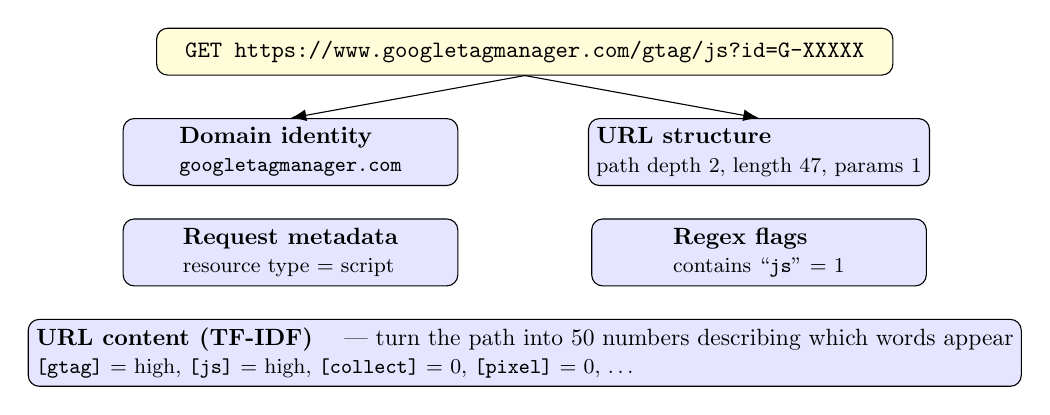
\begin{tikzpicture}[scale=0.85, transform shape]
        \node[draw, rounded corners, fill=yellow!15, minimum width=11cm, minimum height=0.7cm, align=center] (url) at (0, 3) {\texttt{GET https://www.googletagmanager.com/gtag/js?id=G-XXXXX}};

        % Features
        \node[draw, rounded corners, fill=blue!10, minimum width=5cm, minimum height=1cm, align=left] (f1) at (-3.5, 1.5) {\textbf{Domain identity}\\\small \texttt{googletagmanager.com}};
        \node[draw, rounded corners, fill=blue!10, minimum width=5cm, minimum height=1cm, align=left] (f2) at (3.5, 1.5) {\textbf{URL structure}\\\small path depth 2, length 47, params 1};
        \node[draw, rounded corners, fill=blue!10, minimum width=5cm, minimum height=1cm, align=left] (f3) at (-3.5, 0) {\textbf{Request metadata}\\\small resource type = script};
        \node[draw, rounded corners, fill=blue!10, minimum width=5cm, minimum height=1cm, align=left] (f4) at (3.5, 0) {\textbf{Regex flags}\\\small contains ``\texttt{js}'' = 1};
        \node[draw, rounded corners, fill=blue!10, minimum width=11cm, minimum height=1cm, align=left] (f5) at (0, -1.5) {\textbf{URL content (TF-IDF)} \quad — turn the path into 50 numbers describing which words appear\\\small \texttt{[gtag]} = high, \texttt{[js]} = high, \texttt{[collect]} = 0, \texttt{[pixel]} = 0, \dots};

        \draw[-{Latex[length=2mm]}] (url.south) -- (f1.north);
        \draw[-{Latex[length=2mm]}] (url.south) -- (f2.north);
    \end{tikzpicture}

    \vspace{0.3em}
    \small
    \textit{The model takes 80 numbers like this and produces a single bytes-prediction.}
\end{frame}

% ============================================================
% 16 - What's TF-IDF, what's SHAP? (explainer)
% ============================================================
\begin{frame}{Two pieces of jargon, plain English}
    \begin{columns}[T]
    \begin{column}{0.5\textwidth}
        \textbf{\Large TF-IDF}

        \vspace{0.4em}
        \small
        \textit{What words distinguish this URL from others?}

        \vspace{0.5em}
        Tokens like \texttt{gtag}, \texttt{collect}, \texttt{pixel}, \texttt{ad}, \texttt{sync} appear in tracker URLs with very specific frequencies. TF-IDF gives each URL a score on each token. Tokens common across all URLs (like \texttt{com}) are downweighted; tokens that mark a specific kind of resource (like \texttt{gtag}) are upweighted.

        \vspace{0.4em}
        We then compress these scores down to 50 numbers per URL using SVD (a standard dimensionality-reduction trick).
    \end{column}
    \begin{column}{0.5\textwidth}
        \textbf{\Large SHAP}

        \vspace{0.4em}
        \small
        \textit{For one prediction, how much did each feature contribute?}

        \vspace{0.5em}
        Take the model's prediction for one URL. SHAP tells you how much each of the 80 features pushed that prediction up or down, relative to the average.

        \vspace{0.4em}
        Sum SHAP values across many predictions and you get a global picture: \textbf{domain identity drives 48\% of the model's signal, URL content drives 32\%}, the rest is split among the other groups.

        \vspace{0.4em}
        \textit{Different from gain-based importance — gain over-counts high-cardinality features.}
    \end{column}
    \end{columns}
\end{frame}

% ============================================================
% 17 - The data shape and the loss (revisit distribution)
% ============================================================
\begin{frame}{Why the standard loss function is wrong here}
    \begin{columns}[T]
    \begin{column}{0.55\textwidth}
        \centering
        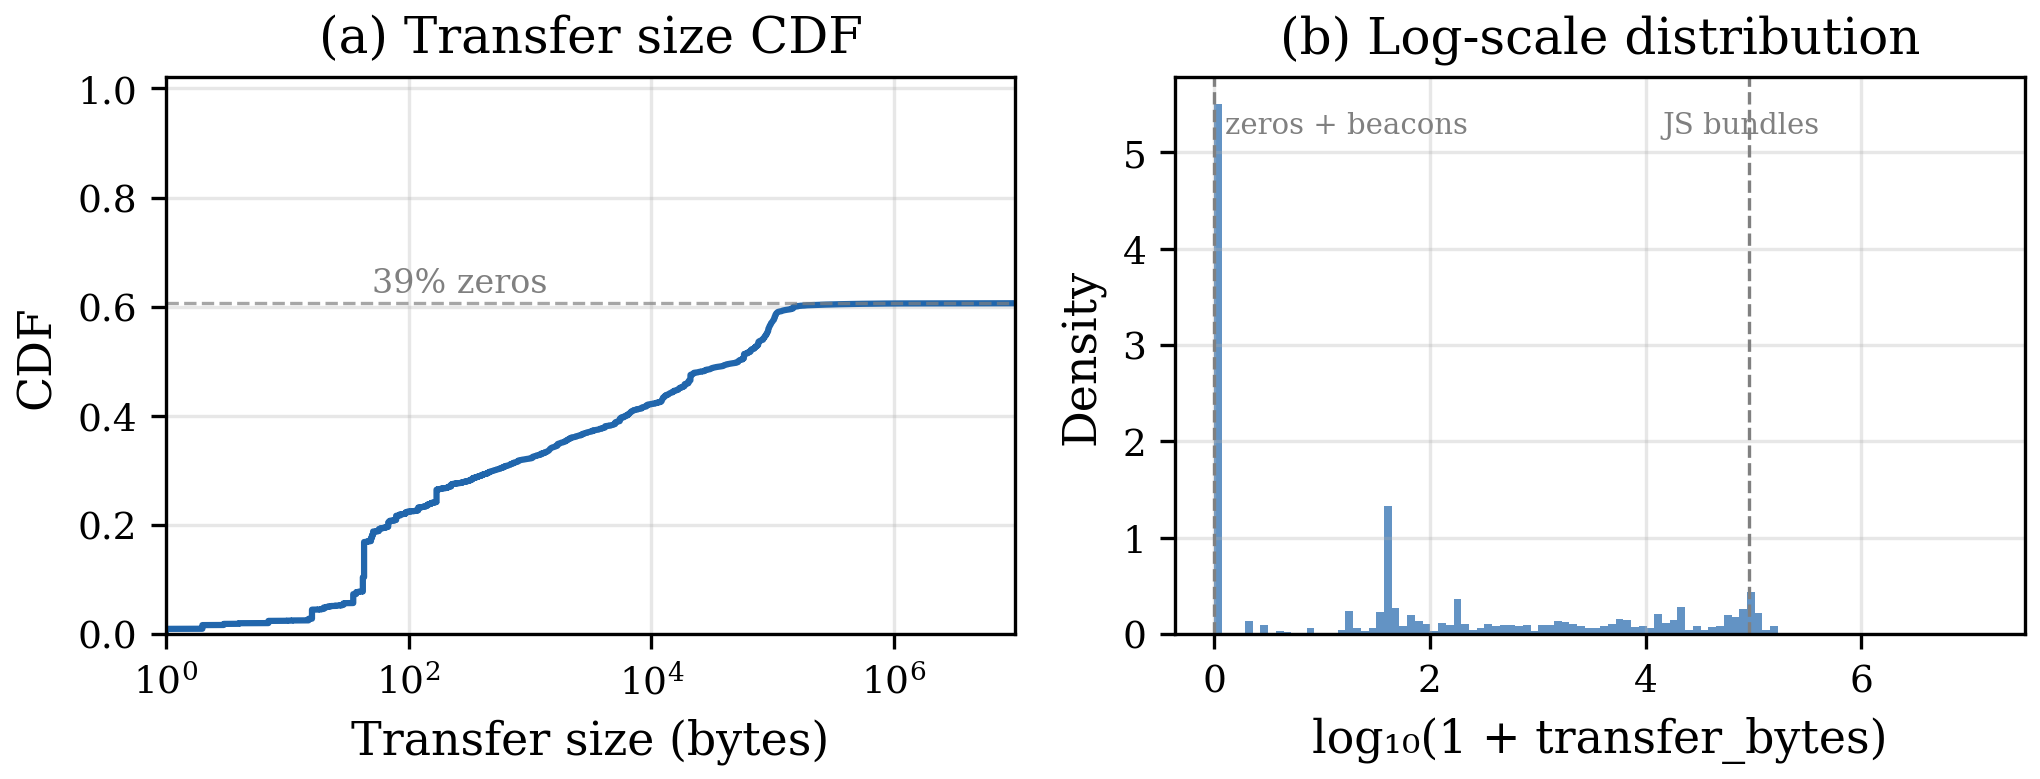
\includegraphics[width=\columnwidth]{figures/fig1_target_distribution.pdf}
    \end{column}
    \begin{column}{0.45\textwidth}
        \small
        \textbf{Squared-error regression assumes} the target is roughly bell-shaped.

        \vspace{0.5em}
        \textbf{Tracker responses are not:} 40\% are zero, the rest heavy-tailed.

        \vspace{0.5em}
        Squared error wastes capacity getting beacons exactly right (zero is easy), and underweights the rare large bundles \textit{that dominate total bandwidth}.

        \vspace{0.5em}
        \textcolor{blue}{We need a loss that natively handles ``spike at zero + long tail.''}
    \end{column}
    \end{columns}
\end{frame}

% ============================================================
% 18 - Tweedie loss (borrow from actuaries)
% ============================================================
\begin{frame}{The loss function: borrow from actuaries}
    \textbf{Web response sizes look just like insurance claims:} \\
    most filings are \$0 (no claim), the rest are heavy-tailed (a few catastrophic claims dominate the total payout). \\
    \textit{40\% of tracker requests return zero bytes (beacons). The rest are heavy-tailed (a few JS bundles dominate the total bandwidth).}

    \vspace{0.8em}
    Actuaries solved this in 1987: \textbf{Tweedie loss} (compound Poisson-Gamma). \\
    A single loss function that handles the spike-at-zero \textit{and} the long tail naturally.

    \vspace{0.8em}
    \small
    Power parameter $p = 1.5$. Sensitivity test: $p \in [1.2, 1.8]$ all within $\pm 4\%$ — the choice is robust.

    \vspace{0.8em}
    \normalsize
    \textcolor{blue}{\textit{The methodological transfer is the contribution.}} \\
    Not "we trained an XGBoost." \textbf{The right loss for the data shape was sitting in another field.}
\end{frame}

% ============================================================
% 19 - Loss function dominates (figure)
% ============================================================
\begin{frame}{The loss function dominates everything else}
    \centering
    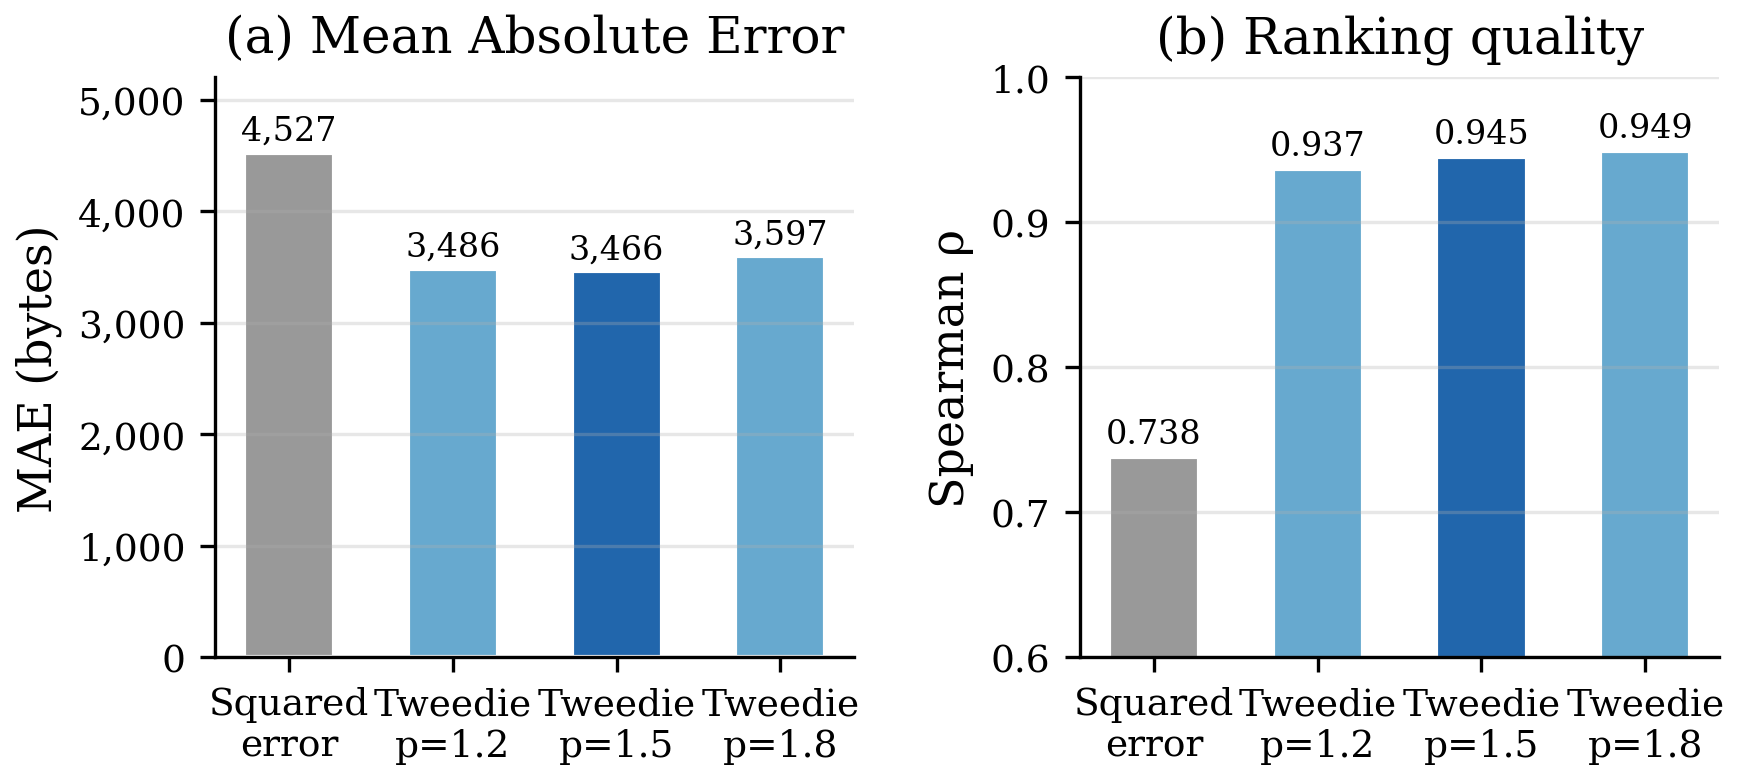
\includegraphics[width=0.7\textwidth]{figures/fig5_loss_ablation.pdf}

    \vspace{0.3em}
    \textbf{Same architecture. Same features. Just swap the loss.} \\
    Squared error: MAE 4{,}527, Spearman 0.74. \quad Tweedie ($p=1.5$): MAE \textbf{3{,}466}, Spearman \textbf{0.95}. \quad \textbf{23\% MAE gap from the loss alone.}

    \vspace{0.3em}
    \small
    \textit{MAE = average bytes off per request. Spearman = how well the model orders cheap-to-expensive (1.0 perfect).} Architecture and feature engineering moved MAE by 4--8\%; the loss moved it 23\%.
\end{frame}

% ============================================================
% 20 - Headline result
% ============================================================
\begin{frame}{Headline result}
    Test set: \textbf{523K requests} (held out from training)

    \vspace{0.5em}
    \begin{table}
        \centering
        \begin{tabular}{lr}
            \toprule
            Method & MAE (bytes) \\
            \midrule
            Global median (everyone gets the same prediction) & 13,661 \\
            Domain LUT & 7,878 \\
            Domain + type LUT (today's status quo for cost estimation) & 6,597 \\
            Path LUT (offline-only, can't deploy at 1.1 GB) & 3,797 \\
            \textbf{XGBoost + Tweedie (ours)} & \textbf{3,466} \\
            \bottomrule
        \end{tabular}
    \end{table}

    \vspace{0.5em}
    \small
    \textbf{47.5\% MAE reduction} over the deployable LUT baseline. \\
    Bootstrap confidence intervals (resample test set 1{,}000$\times$, see how stable the number is): model CI does \textbf{not} overlap path LUT CI. The improvement is real, not noise.

    \vspace{0.4em}
    \normalsize
    \textcolor{blue}{But this number understates the actual finding.}
\end{frame}

% ============================================================
% 21 - Path decomposition
% ============================================================
\begin{frame}{The model wins even where the LUT \textit{has the answer}}
    \begin{columns}[T]
    \begin{column}{0.55\textwidth}
        \centering
        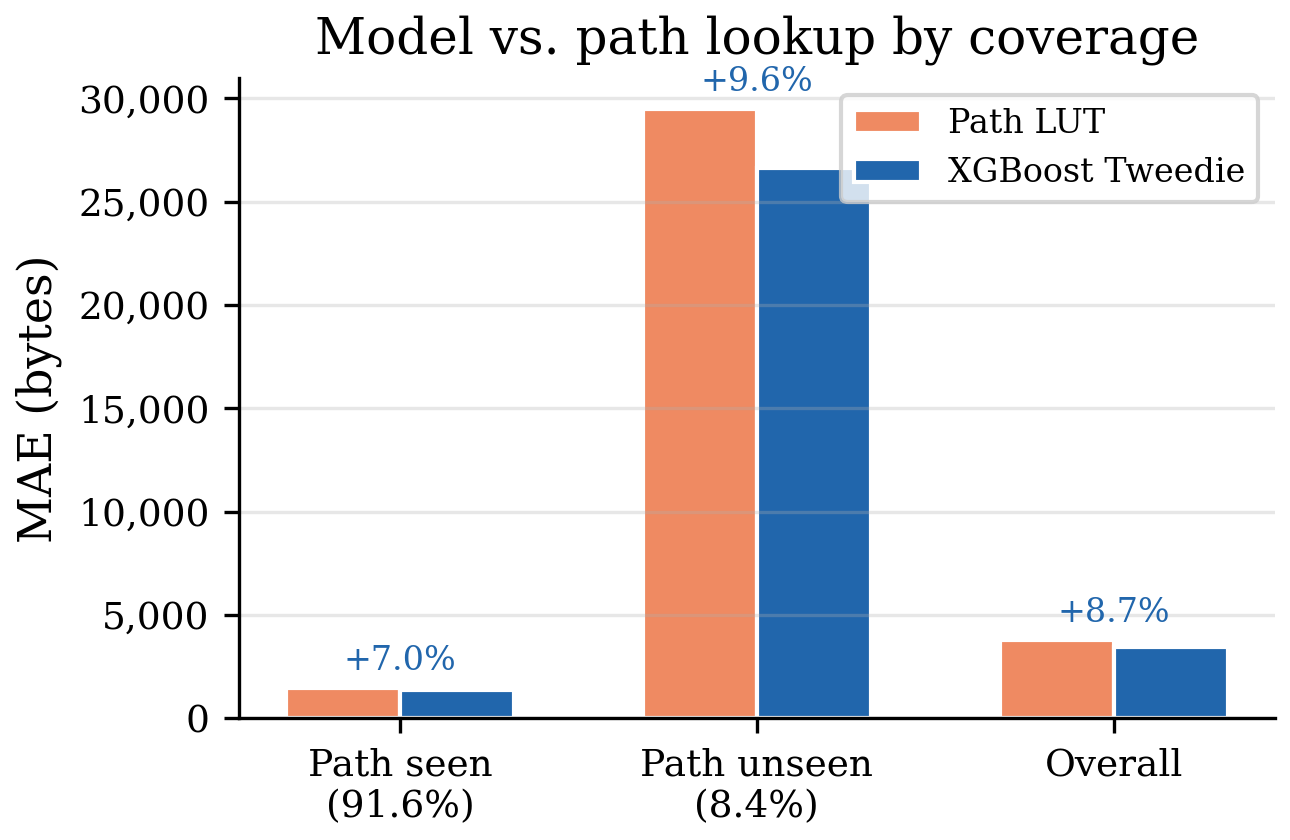
\includegraphics[width=\columnwidth]{figures/fig9_path_decomposition.pdf}
    \end{column}
    \begin{column}{0.45\textwidth}
        Split test set by whether the path was \textbf{seen in training}:

        \vspace{0.7em}
        \textbf{Path seen} (91.6\% of rows):
        \begin{itemize}
            \item Path LUT: 1{,}448 bytes MAE
            \item Model: \textbf{1{,}346 bytes MAE}
        \end{itemize}

        \vspace{0.4em}
        \small
        Confidence intervals don't overlap — statistically significant.

        \vspace{0.7em}
        \normalsize
        \textcolor{blue}{The model isn't winning on unseen paths.} \\
        \textbf{It's winning on \textit{seen} paths by regularizing.}

        \vspace{0.4em}
        Even where the lookup has the exact answer memorized, the model still wins.
    \end{column}
    \end{columns}
\end{frame}

% ============================================================
% 22 - Aggregation (figure)
% ============================================================
\begin{frame}{What the user actually sees: weekly aggregates}
    \begin{columns}[T]
    \begin{column}{0.55\textwidth}
        \centering
        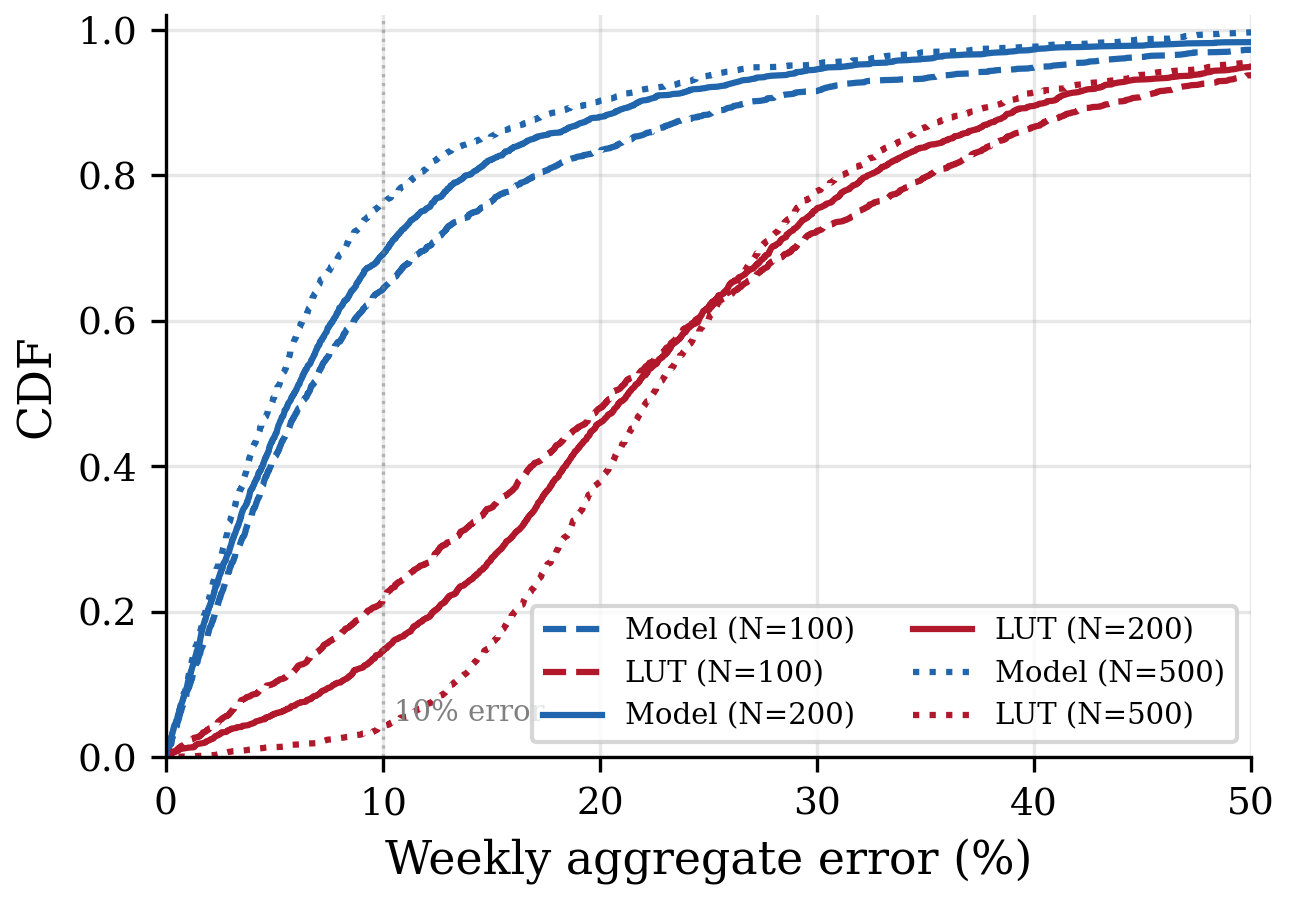
\includegraphics[width=\columnwidth]{figures/fig3_aggregation_cdf.pdf}
    \end{column}
    \begin{column}{0.45\textwidth}
        Users don't see per-request predictions. They see \textbf{weekly totals}.

        \vspace{0.7em}
        At $N = 200$ blocked requests/week (moderate browsing):
        \begin{itemize}
            \item Domain+type LUT: \textbf{22\%} median error
            \item \textbf{Our model: 6\%}
        \end{itemize}

        \vspace{0.7em}
        \textbf{68.5\% of weeks within 10\%} of true cost.

        \vspace{0.7em}
        Per-request noise cancels. \\
        LUT errors are \textbf{systematic biases that compound}.
    \end{column}
    \end{columns}
\end{frame}

% ============================================================
% 23 - Why noise cancels (visual explainer)
% ============================================================
\begin{frame}{Why per-request noise cancels (and LUT bias doesn't)}
    \centering
    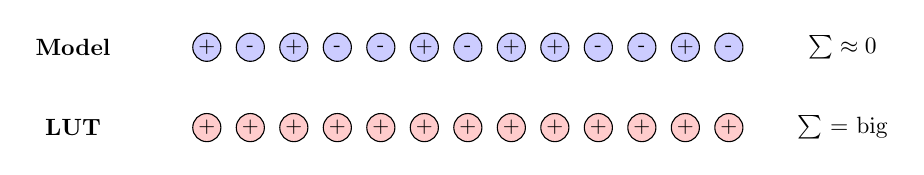
\begin{tikzpicture}[scale=0.85, transform shape]
        % Model row
        \node at (-6.5, 1.2) {\textbf{Model}};
        \foreach \i/\v in {0/+,1/-,2/+,3/-,4/-,5/+,6/-,7/+,8/+,9/-,10/-,11/+,12/-} {
            \node[draw, circle, fill=blue!20, minimum size=0.42cm, inner sep=0pt, font=\small] at (-4.5 + 0.65*\i, 1.2) {\v};
        }
        \node at (5, 1.2) {$\sum \approx 0$};

        % LUT row
        \node at (-6.5, 0) {\textbf{LUT}};
        \foreach \i/\v in {0/+,1/+,2/+,3/+,4/+,5/+,6/+,7/+,8/+,9/+,10/+,11/+,12/+} {
            \node[draw, circle, fill=red!20, minimum size=0.42cm, inner sep=0pt, font=\small] at (-4.5 + 0.65*\i, 0) {\v};
        }
        \node at (5, 0) {$\sum$ = big};
    \end{tikzpicture}

    \vspace{0.3em}
    \small
    \textbf{Model:} per-request errors switch sign — they cancel in a weekly sum.\\
    \textbf{LUT:} errors point the same direction (consistently over- or under-predicts certain URL patterns) — they accumulate.

    \vspace{0.4em}
    \textcolor{blue}{This is why the model's advantage \textit{widens} with more requests per week — and why the LUT's per-request accuracy is misleading.}
\end{frame}

% ============================================================
% 24 - Resource type breakdown (figure)
% ============================================================
\begin{frame}{Where the wins concentrate: by resource type}
    \centering
    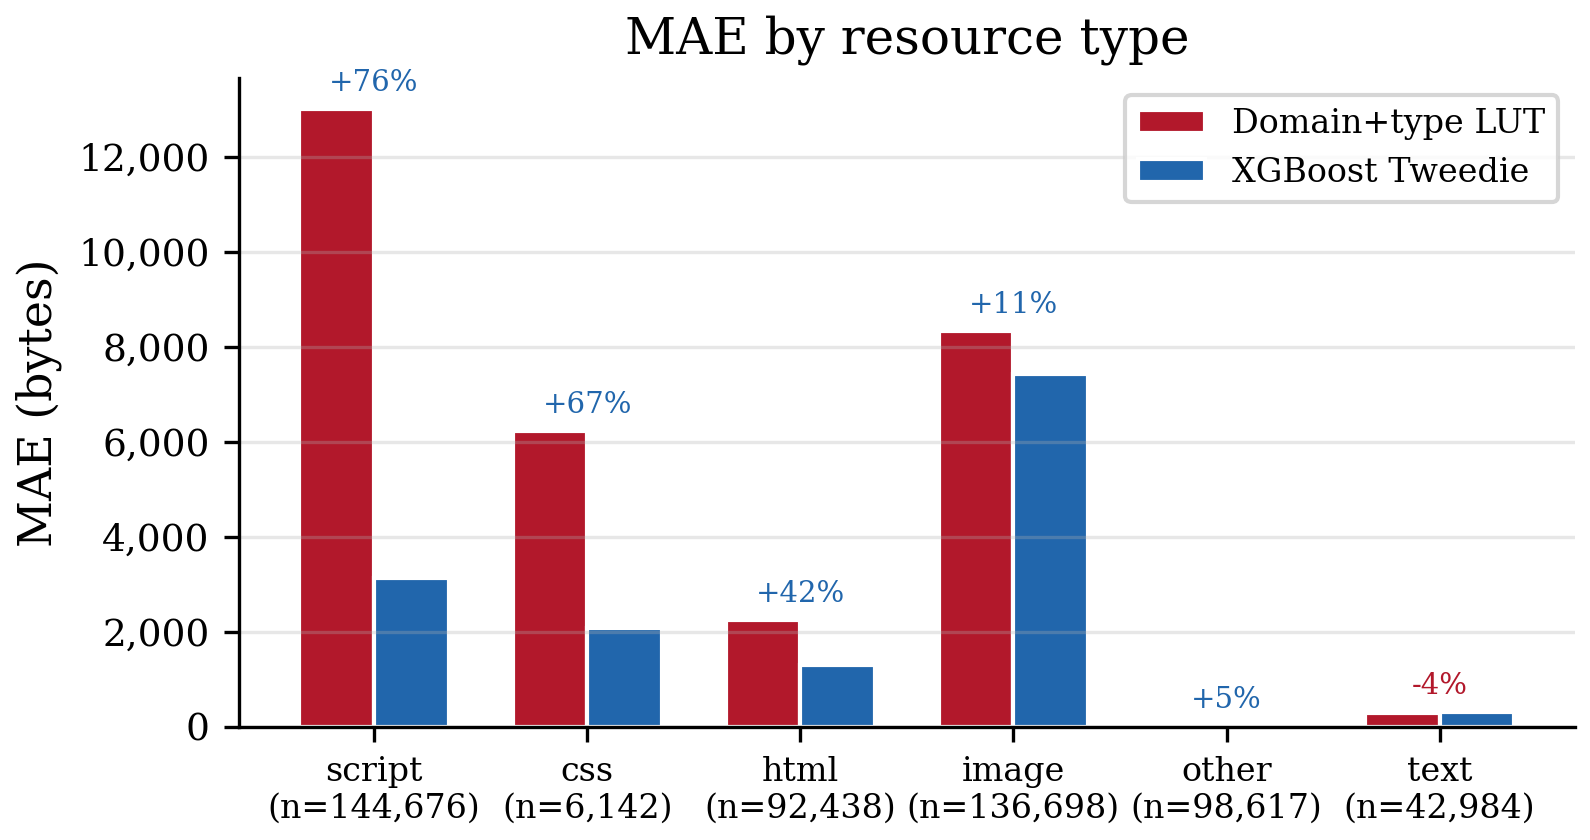
\includegraphics[width=0.72\textwidth]{figures/fig4_per_resource_type.pdf}

    \vspace{0.2em}
    \small
    \textbf{Scripts (+76\%) and CSS (+67\%)} are where the model crushes the LUT — also the \textit{high-cost} resources that dominate weekly bandwidth. Beacons (+5\%) and text are unchanged because the LUT was already near-optimal for low-variance types.

    \vspace{0.2em}
    \textcolor{blue}{The model's gains land exactly where bandwidth actually goes.}
\end{frame}

% ============================================================
% 25 - Multi-target aggregation (figure)
% ============================================================
\begin{frame}{Aggregation rescues even noisy targets}
    \centering
    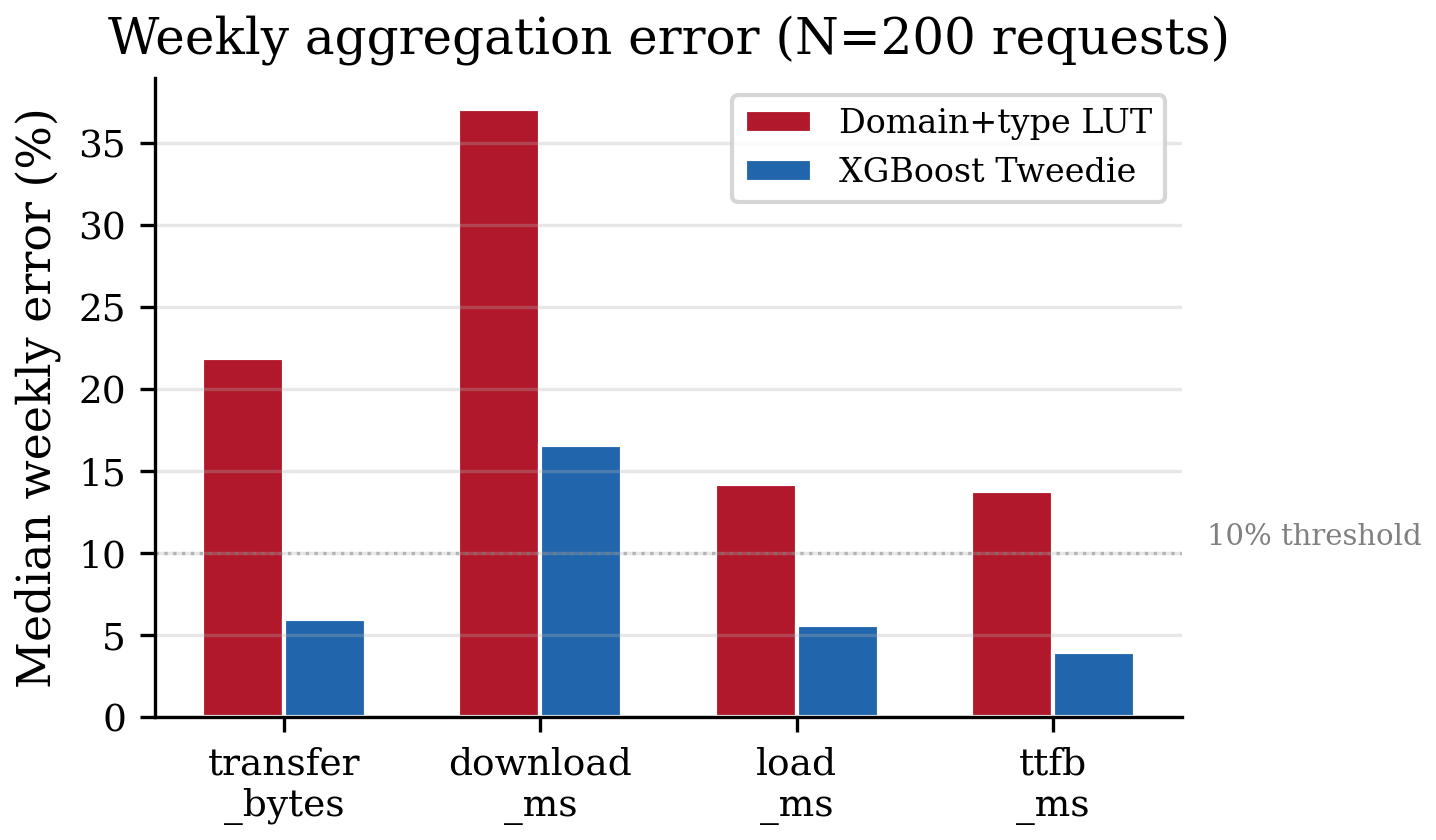
\includegraphics[width=0.72\textwidth]{figures/fig10_multi_target_agg.pdf}

    \vspace{0.2em}
    \small
    Per-request, the model is \textit{worse} than the LUT on TTFB and load time (timing is network-dependent, not URL-dependent). \textbf{But in weekly aggregation, the model wins on all four targets.} LUT bias compounds; model noise cancels.

    \vspace{0.2em}
    \textcolor{blue}{Aggregate accuracy depends on \textit{bias}, not per-request noise.}
\end{frame}

% ============================================================
% 26 - Robustness (correlated browsing + temporal)
% ============================================================
\begin{frame}{Does it hold up in realistic conditions? Yes.}
    \textbf{Domain-correlated browsing} (real users return to the same sites — uniform random sampling is unrealistic):
    \begin{itemize}
        \item Domain+type LUT: 36.4\% weekly error
        \item \textbf{Our model: 12.9\% weekly error}
        \item Model's advantage \textit{widens} when browsing is concentrated
    \end{itemize}

    \vspace{0.8em}
    \textbf{Temporal generalization} (train June 2024, test September 2024 — 3 months later):
    \begin{itemize}
        \item Both methods degrade $\sim$30\% as URL space evolves
        \item \textbf{Model retains a 33\% advantage} over LUT
        \item Recommended retraining cadence: \textbf{quarterly}
    \end{itemize}
\end{frame}

% ============================================================
% 27 - Deployment status
% ============================================================
\begin{frame}{Deployment status}
    \textbf{Integration into Firefox's new-tab privacy widget is \textit{planned}}, not yet scheduled.

    \vspace{0.8em}
    \textbf{Proposed integration:}
    \begin{itemize}
        \item \textbf{Distribution:} Remote Settings (model updates without browser releases)
        \item \textbf{Inference path:} alongside the existing block decision -- no impact on the hot path
        \item \textbf{Features:} all available via \texttt{nsIChannel} and \texttt{nsILoadInfo} at block time -- \textbf{no new instrumentation}
        \item \textbf{Retraining:} quarterly on fresh HTTP Archive crawls
        \item \textbf{Artifact:} $\sim$500 KB ONNX ($\sim$2 MB with TF-IDF vocab)
    \end{itemize}

    \vspace{0.5em}
    \small
    Production browsers today (Firefox, Brave, Safari, Chrome) all surface tracker blocks as \textbf{counts}. Brave's prior work was page-level research, not per-request. The per-request cost primitive is what's new here.
\end{frame}

% ============================================================
% 28 - Limitations
% ============================================================
\begin{frame}{Limitations and honest caveats}
    \textbf{Deploy transfer size + download duration only.} Timing metrics like TTFB and total page load depend heavily on network and device — HTTP Archive crawls from a fixed test environment, so timing predictions don't transfer cleanly to real users.

    \vspace{0.5em}
    \textbf{Cascading effects.} Blocking a tag manager prevents downstream injected requests we never see. Predictions are a \textbf{lower bound} on true bandwidth saved.

    \vspace{0.5em}
    \textbf{Server-side variation.} A/B tests, geo-targeting, SDK versioning all make the same URL return different bytes on different requests. Irreducible per-request noise. Aggregation mitigates.

    \vspace{0.5em}
    \textbf{The model makes no blocking decisions.} The Disconnect list decides what to block. Our model only estimates the cost of an already-decided block. A miscalibrated estimate produces a misleading aggregate, never an over-block or under-block.

    \vspace{0.5em}
    \textbf{Adversarial robustness out of scope.} Threat model is \textit{honest measurement}, not evasion.
\end{frame}

% ============================================================
% 29 - Takeaways
% ============================================================
\begin{frame}{Takeaways}
    \begin{enumerate}
        \item \textbf{Within-domain transfer size varies by 3 orders of magnitude.} The URL path -- not the domain -- is the primary cost determinant.

        \vspace{0.4em}
        \item \textbf{Tweedie loss beats squared error by 23\%} on identical features. Loss function selection dominates architecture and feature engineering for this kind of data.

        \vspace{0.4em}
        \item \textbf{The model beats exact-path lookup on seen paths.} Regularization across URL structure beats memorization.

        \vspace{0.4em}
        \item \textbf{6\% weekly aggregation error.} Per-request noise cancels; LUT biases compound. The widget becomes honest.

        \vspace{0.4em}
        \item \textbf{Deploys via Remote Settings.} Same channel as the blocklist. No new instrumentation. No hot-path impact. 2{,}000$\times$ smaller than the path LUT.
    \end{enumerate}
\end{frame}

% ============================================================
% 30 - Thanks
% ============================================================
\begin{frame}{Thanks}
    \textbf{Tim} for the advising work. \\
    \textbf{Privacy team} for the guidance.

    \vspace{2em}
    \begin{center}
        \Large{Questions?}
    \end{center}
\end{frame}

\end{document}
